\section{Transformer}
Transformer is a deep learning architecture showed in figure \ref{fig:transformer} that was introduced in 2017 by Vaswani et al \cite{NIPS2017_3f5ee243}. It builds on the ideas presented in two influential researchs, sequence to sequence \cite{NIPS2014_a14ac55a, DBLP:journals/corr/WuSCLNMKCGMKSJL16} and attention mechanism \cite{luong-etal-2015-effective}, and has become the state-of-the-art architecture for various natural language processing tasks.\\\\
The Transformer Encoder is composed of multiple layers. The first layer is Multi-head Attention, and the second layer is Position-wise Feed-forward network. In the Encoder Self-Attention, Queries, Keys, and Values are all derived from the outputs of the previous Encoder Layer. Both sublayers use a residual connection, inspired by the ResNet architecture \cite{he2016deep}. This additional residual connection is immediately followed by Layer Normalization \cite{ba2016layer}. As a result, the Transformer Encoder produces a vector representation for each position of the input sequence.\\\\
The Transformer Decoder is also a stack of multiple layers. In addition to the two sublayers described in the Encoder, the Decoder includes a third sublayer called the Encoder-Decoder Attention, or Cross-Attention, between these two. In the Encoder-Decoder Attention, Queries are derived from the outputs of the previous Decoder Layer, while the Keys and Values are derived from the Transformer Encoder outputs. In the Decoder Self-Attention, Queries, Keys, and Values are derived from the outputs of the previous Decoder Layer. However, each position in the Decoder can only attend to all positions in the Decoder up to that position, which is called Masked Self-Attention. This Masked Self-Attention preserves the autoregressive property, ensuring that the prediction only depends on those output tokens that have been generated.\\\\
In summary, the transformer model is a powerful and flexible architecture that owes its success to the combination of the sequence to sequence learning approach and the attention mechanism.\\\\ 
\begin{figure}[hbt]
    \centering
    
    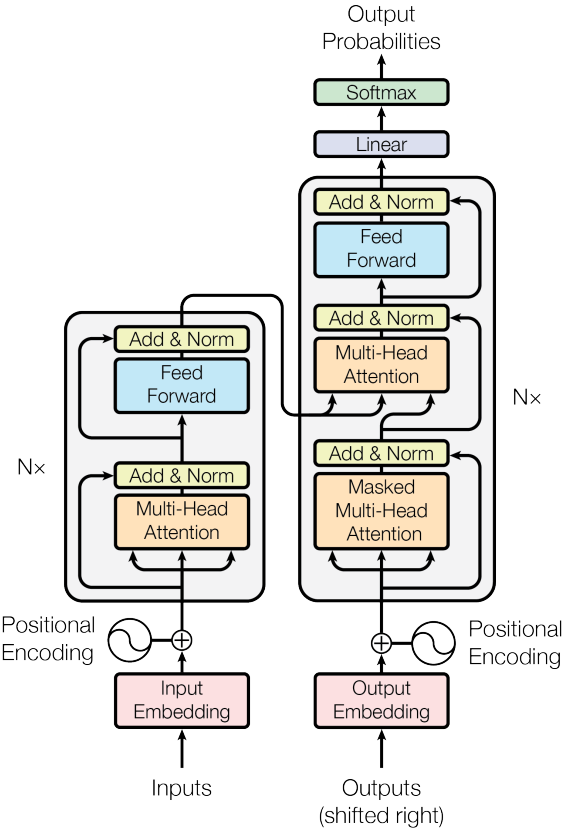
\includegraphics[width=0.6\textwidth]{theoretical-background/image/transformer.png}
    \caption{The architecture of transformers presented in the research paper "Attention is all you need" \cite{NIPS2017_3f5ee243}}
    \label{fig:transformer}
\end{figure}
\textbf{Scaled Dot-Product Attention}: It computes how much each value vector contributes to the output vector, based on the similarity between the query vector Q and the key vector Q. The similarity is measured by the dot product, which is scaled down by the square root of the dimension of the key vector $d_k$. The scaled dot products are then normalized by a softmax function to get the attention weights. The output vector is the weighted sum of the value vectors.
\begin{align}
    Attention (Q,K,V)=softmax(\frac{QK^T}{\sqrt(d_k)})V
\end{align}

\textbf{Multi-head Attention}: It applies the attention function multiple times in parallel, each of them is called a head, using different projections of the query, key and value vectors. This allows the model to capture different aspects of the input and output sequences. The outputs of the multi-head attention are concatenated and projected to get the final output.
\begin{align}
    MultiHead(Q,K,V)= Concat(head_1,...,head_h)W^O\\
    \text{where } head_i=Attention(QW_{i}^Q, KW_{i}^K, VW_{i}^V)
\end{align}

\textbf{Position-wise Feed-forward Networks}: This is a way of transforming the output of the attention layers using a simple neural network that consists of two linear layers with a ReLU activation in between. The network is applied to each position separately and identically, meaning that it does not depend on the order of the sequence. The network has the same input and output dimension as the attention layers, but a larger hidden dimension.
\begin{align}
    FFN(x)=max(0,x\cdot W_1+b_1)\cdot W_2+b_2
\end{align}
